\section{Lab 2}
\subsection{Exercise 2.1}
\lstinputlisting[language=Prolog]{./2/ex1.pl}
\pagebreak
\subsubsection{Queries}
\begin{lstlisting}[language=Prolog]
| ?- sorted([1,2,3]).
yes
| ?- sorted([1,3,2]).
no
| ?- qsort([2,5,1,6,8,3,4], Sorted).
Sorted = [1,2,3,4,5,6,8] ? ;
no
| ?- ssort([2,5,1,6,8,3,4], Sorted).
Sorted = [1,2,3,4,5,6,8] ? ;
no
\end{lstlisting}
\subsection{Exercise 2.2}
\lstinputlisting[language=Prolog]{./2/ex2.pl}
\pagebreak
\subsubsection{Questions}
\begin{itemize}
  \item Examine how the execution of the following queries is affected by the ordering
  of the clauses and the premises within clauses.
  \begin{lstlisting}[language=Prolog]
    | ?- middle(X, [a,b,c]).
    | ?- middle(a, X).
  \end{lstlisting}
  Try all four possible permutations of middle/2 and (1) explain what happens,
  (2) why and (3) sketch the SLD tree (you don’t have to draw the whole
  tree...). Don’t forget to explain what happens when you ask for more than
  one answer! Which version is preferable for each type of query?
\end{itemize}
\begin{enumerate}
  \item The execution path will differ between permutations. This is because Prolog choses which premise to be resolved depending on the order in the rule and which rule or fact to use depending on the ordering of the program's rules and facts.
  \item For the program - a rule or fact that precedes (read top to down) another rule or fact with the same name and arity will be used first. For the premises of a rule - a premise that precedes (read left-right) another premise will be resolved first.
  \item The SLD-trees for each permutation and query is drawn in figure \ref{xabc}, \ref{cx1} and \ref{cx2}. An underlined clause is selected for resolving. A successful leaf is marked with $\blacksquare$ and an unsuccessful with $\square$.
  
  When asked for additional answers Prolog backtracks from the last given answer to the next closest possibility. For instance, in figure \ref{m1xabc} the first given answer is the leftmost leaf, when asked for more answers Prolog backtracks, tries the other rule for the query which is unsuccessful. Prolog then backtracks all the way to the root since no other possible branches are found on.

  Because of Prolog's selection rule the leftmost child of an SLD-tree is reached first. This means that middle1 (figure \ref{m1xabc}) is the most efficient permutation for the query middle(X, [a,b,c]). Although middle3 (figure \ref{m3xabc}) reaches the first answer as quickly as middle1 it will continue to loop forever if we ask for more answers. This is due to the ordering of the clauses of middle3. Middle is always an unconstrained variable which, in this case, produces an infinite number of possibilities to try.

  The most efficient permutation for middle(a, X) is middle3 which always reaches a successful leaf (neglecting what happens during the resolving of append). All permutations for this query except middle4 produces an infinite amount of answers. Middle4 never reaches a leaf.


\end{enumerate}

\begin{figure}[H]
  \centering
  \subfloat[{middle1(X, [a,b,c])}]{\label{m1xabc}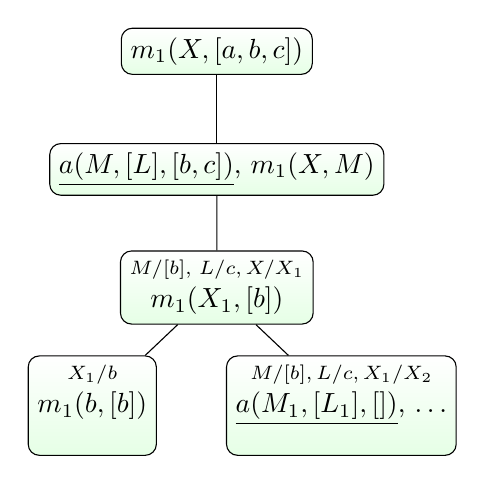
\begin{tikzpicture}[sibling distance=9em, align=center,
  every node/.style = {shape=rectangle, rounded corners,
    draw, align=center,
    top color=white, bottom color=green!10}]]
  \node {$m_1(X,[a,b,c])$}
    child { node {\underline{$a(M, [L], [b,c])$}, $m_1(X, M)$}
      child { node {\scriptsize $M/[b]$, $L/c, X/X_1$\\$m_1(X_1, [b])$}
        child { node {\scriptsize $X_1/b$\\ $m_1(b, [b])$\\$\blacksquare$}}
        child { node {\scriptsize $M/[b], L/c, X_1/X_2$\\\underline{$a(M_1, [L_1], [])$}, $\ldots$\\$\square$}}
      }
    };
\end{tikzpicture}}\hspace{0.5cm} 
  \subfloat[{middle2(X, [a,b,c])}]{\label{m2xabc}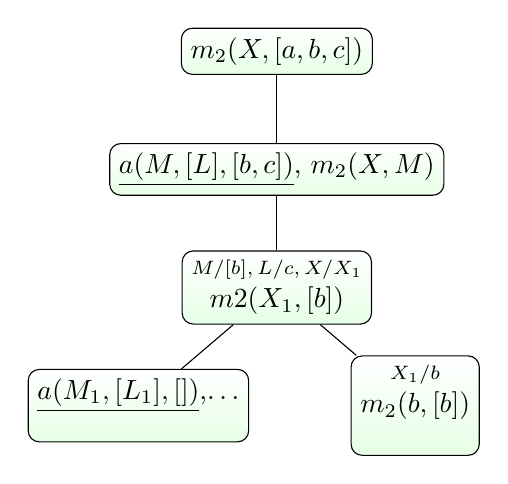
\begin{tikzpicture}[sibling distance=10em, align=center,
  every node/.style = {shape=rectangle, rounded corners,
    draw, align=center,
    top color=white, bottom color=green!10}]]
  \node {$m_2(X,[a,b,c])$}
    child { node {\underline{$a(M, [L], [b,c])$}, $m_2(X, M)$}
      child { node {\scriptsize $M/[b], L/c, X/X_1$\\$m2(X_1, [b])$}
        child { node {\underline{$a(M_1,[L_1],[])$},$\ldots$\\$\square$}}
        child { node {\scriptsize $X_1/b$\\$m_2(b, [b])$\\$\blacksquare$}}
      }
    };
\end{tikzpicture}}\\
  \subfloat[{middle3(X, [a,b,c])}]{\label{m3xabc}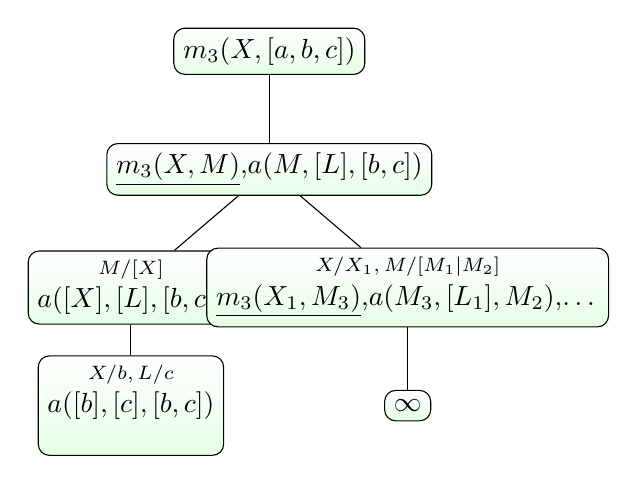
\begin{tikzpicture}[sibling distance=10em,
    every node/.style = {shape=rectangle, rounded corners,
      draw, align=center,
      top color=white, bottom color=green!10}]]
    \node {$m_3(X,[a,b,c])$}
      child { node {\underline{$m_3(X, M)$},$a(M, [L], [b,c])$}
        child { node {\scriptsize $M/[X]$\\$a([X], [L], [b,c])$}
          child { node {\scriptsize $X/b, L/c$\\$a([b],[c],[b,c])$\\$\blacksquare$}}
        }
        child {node {\scriptsize $X/X_1, M/[M_1|M_2]$\\\underline{$m_3(X_1,M_3)$},$a(M_3,[L_1],M_2)$,\ldots}
          child {node {$\infty$}}
        }
      };
  \end{tikzpicture}}\hspace{0.2cm}
  \subfloat[{middle4(X, [a,b,c])}]{\label{m4xabc}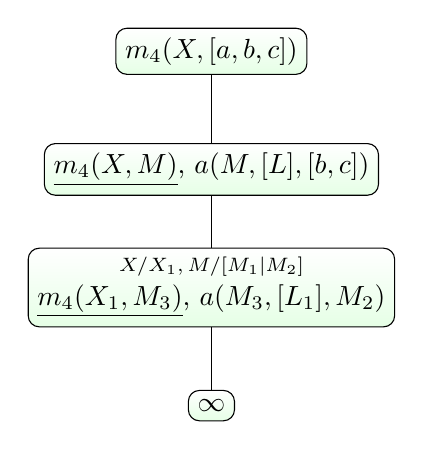
\begin{tikzpicture}[sibling distance=10em,
  every node/.style = {shape=rectangle, rounded corners,
    draw, align=center,
    top color=white, bottom color=green!10}]]
  \node {$m_4(X,[a,b,c])$}
    child { node {\underline{$m_4(X, M)$}, $a(M, [L], [b,c]$)}
      child { node {\scriptsize $X/X_1, M/[M_1|M_2]$\\\underline{$m_4(X_1, M_3)$}, $a(M_3, [L_1], M_2)$}
        child { node {$\infty$}}
      }
    };
\end{tikzpicture}}
  \caption{SLD-trees for queries with the arguments (X, [a,b,c])}
  \label{xabc}
\end{figure}

\begin{figure}[H]
  \begin{adjustwidth}{\oddsidemargin-0.8in}{-\rightmargin}    
  \subfloat[{middle1(c, X)}]{\label{m1xabc}% % Permutation 1
% middle1(X, [X]).
% middle1(X, [First|Xs]) :-
%  append(Middle, [Last], Xs),
%  middle1(X, Middle).

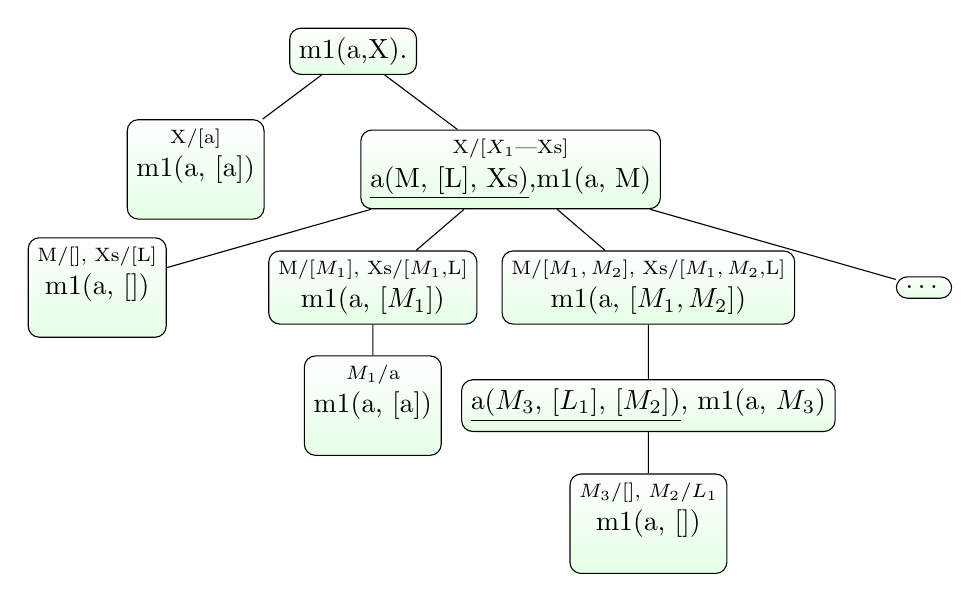
\begin{tikzpicture}[sibling distance=12em, align=center,
  every node/.style = {shape=rectangle, rounded corners,
    draw, align=center,
    top color=white, bottom color=green!10},
    level 1/.style={sibling distance=4cm},
    level 2/.style={sibling distance=3.5cm}, 
    level 3/.style={sibling distance=3cm}, ]
  \node {m1(a,X).}
    child { node {\scriptsize X/[a]\\m1(a, [a])\\$\blacksquare$}}
    child { node {\scriptsize X/[$X_1$|Xs]\\\underline{a(M, [L], Xs)},m1(a, M)}
      child { node {\scriptsize M/[], Xs/[L]\\m1(a, [])\\$\square$}}
      child { node {\scriptsize M/[$M_1$], Xs/[$M_1$,L]\\m1(a, [$M_1$])}
        child { node {\scriptsize $M_1$/a\\m1(a, [a])\\$\blacksquare$}}  
      }
      child { node {\scriptsize M/[$M_1,M_2$], Xs/[$M_1,M_2$,L]\\m1(a, [$M_1,M_2$])}
        child { node {\underline{a($M_3$, [$L_1$], $[M_2]$)}, m1(a, $M_3$)}
          child {node {\scriptsize $M_3$/[], $M_2/L_1$\\m1(a, [])\\$\square$}}
        }
      }
      child {node {\ldots}}
    };
\end{tikzpicture}}\\
  \end{adjustwidth}
  \begin{adjustwidth}{-\oddsidemargin-0.15in}{-\rightmargin}        
  \vspace{1cm}\subfloat[{middle2(c, X)}]{\label{m2xabc}% % Permutation 2
% middle2(X, [First|Xs]) :-
% append1(Middle, [Last], Xs),
% middle2(X, Middle).
% middle2(X, [X]).

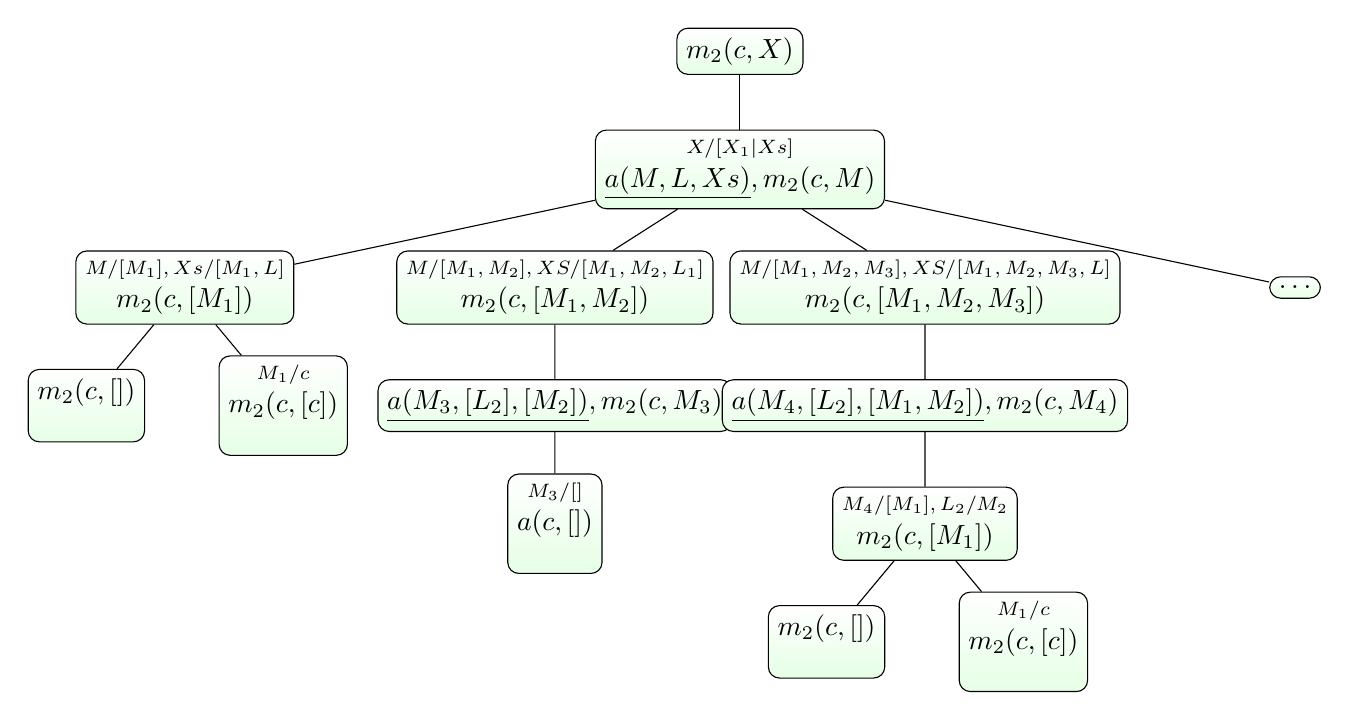
\begin{tikzpicture}[sibling distance=12em, align=center,
  every node/.style = {shape=rectangle, rounded corners,
    draw, align=center,
    top color=white, bottom color=green!10},
    level 1/.style={sibling distance=4cm},
    level 2/.style={sibling distance=4.7cm}, 
    level 3/.style={sibling distance=2.5cm}, ]
  \node {$m_2(c,X)$}
    child { node {\scriptsize $X/[X_1|Xs]$\\$\underline{a(M,L,Xs)},m_2(c,M)$}
      child { node {\scriptsize $M/[M_1], Xs/[M_1,L]$\\$m_2(c, [M_1])$}
        child { node { $m_2(c,[])$\\ $\square$}}
        child { node { \scriptsize $M_1/c$\\ $m_2(c, [c])$\\$\blacksquare$}}
      }
      child { node {\scriptsize $M/[M_1,M_2], XS/[M_1,M_2,L_1]$\\$m_2(c,[M_1,M_2])$}
        child { node {$\underline{a(M_3, [L_2], [M_2])},m_2(c, M_3)$}
          child { node {\scriptsize$M_3/[]$\\$a(c,[])$\\$\square$}}
        }
      }
      child { node {\scriptsize $M/[M_1,M_2,M_3],XS/[M_1,M_2,M_3,L]$\\$m_2(c,[M_1,M_2,M_3])$}
        child { node {$\underline{a(M_4,[L_2],[M_1,M_2])},m_2(c,M_4)$}
          child { node {\scriptsize $M_4/[M_1], L_2/M_2$\\$m_2(c,[M_1])$}
            child { node {$m_2(c, [])$\\$\square$}}
            child { node {\scriptsize $M_1/c$\\$m_2(c, [c])$\\$\blacksquare$}}
          }
        }
      }
      child {node {$\ldots$}}
    };
\end{tikzpicture}}\\
  \end{adjustwidth}
  \caption{SLD-trees for queries with the arguments (c, X)}
  \label{cx1}
\end{figure}

\begin{figure}[H]
  \begin{adjustwidth}{\oddsidemargin-1.5in}{-\rightmargin}
  \subfloat[{middle3(c, X)}]{\label{m3xabc}% % Permutation 3
% middle3(X, [X]).
% middle3(X, [First|Xs]) :-
%   middle3(X, Middle),
%   append1(Middle, [Last], Xs).

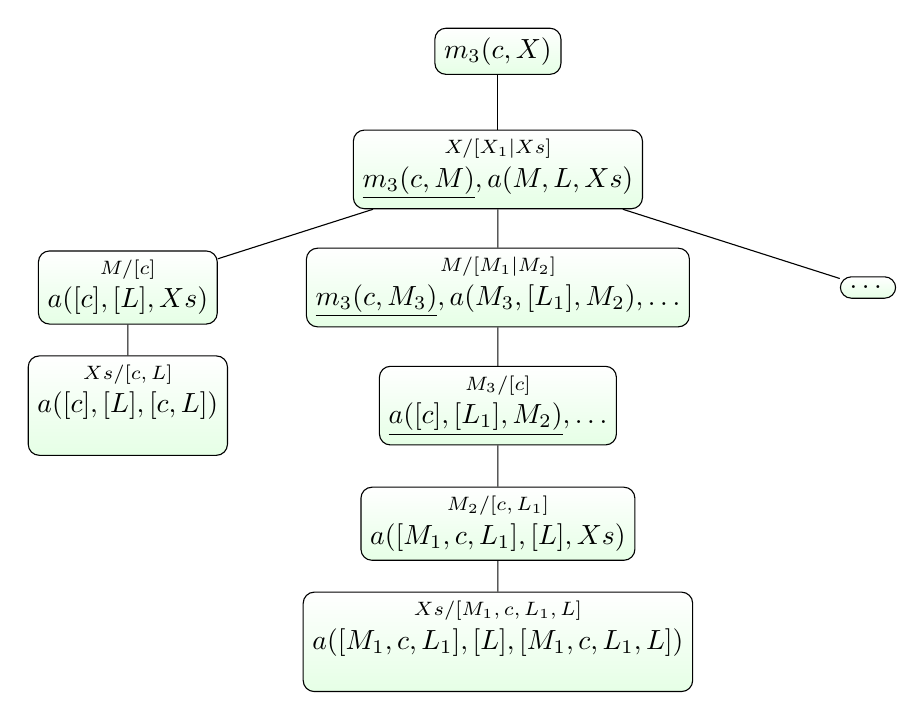
\begin{tikzpicture}[sibling distance=12em, align=center,
  every node/.style = {shape=rectangle, rounded corners,
    draw, align=center,
    top color=white, bottom color=green!10},
    level 1/.style={sibling distance=4cm},
    level 2/.style={sibling distance=4.7cm}, 
    level 3/.style={sibling distance=2.5cm}, ]
  \node {$m_3(c,X)$}
    child { node {\scriptsize $X/[X_1|Xs]$\\$\underline{m_3(c,M)},a(M,L,Xs)$}
      child {node {\scriptsize $M/[c]$\\$a([c],[L],Xs)$}
        child {node {\scriptsize $Xs/[c,L]$\\$a([c],[L],[c,L])$\\$\blacksquare$}}
      }
      child { node {\scriptsize $M/[M_1|M_2]$\\$\underline{m_3(c,M_3)},a(M_3,[L_1],M_2),\ldots$}
        child { node {\scriptsize $M_3/[c]$\\$\underline{a([c],[L_1],M_2)},\ldots$}
          child { node {\scriptsize $M_2/[c,L_1]$\\$a([M_1,c,L_1],[L],Xs)$}
            child {node {\scriptsize $Xs/[M_1,c,L_1,L]$\\$a([M_1,c,L_1],[L],[M_1,c,L_1,L])$\\$\blacksquare$}}
          }
        }
      }
      child { node {\ldots}}
    };
\end{tikzpicture}}
  \subfloat[{middle4(c, X)}]{\label{m4xabc}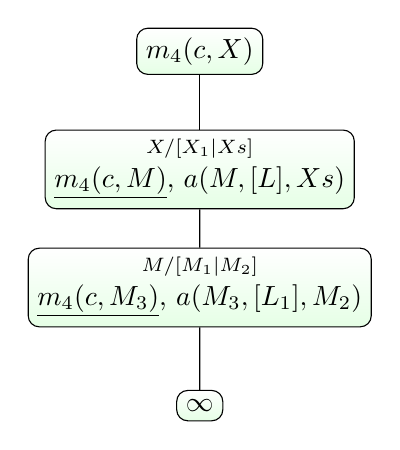
\begin{tikzpicture}[sibling distance=12em, align=center,
  every node/.style = {shape=rectangle, rounded corners,
    draw, align=center,
    top color=white, bottom color=green!10},
    level 1/.style={sibling distance=4cm},
    level 2/.style={sibling distance=4.7cm}, 
    level 3/.style={sibling distance=2.5cm}, ]
    \node {$m_4(c,X)$}
    child { node {\scriptsize $X/[X_1|Xs]$\\\underline{$m_4(c, M)$}, $a(M, [L], Xs$)}
      child { node {\scriptsize $M/[M_1|M_2]$\\\underline{$m_4(c, M_3)$}, $a(M_3, [L_1], M_2)$}
        child { node {$\infty$}}
      }
    };
\end{tikzpicture}}
  \end{adjustwidth}
  \caption{SLD-trees for queries with the arguments (c, X)}
  \label{cx2}
\end{figure}

\pagebreak

\subsection{Exercise 2.3}
\lstinputlisting[language=Prolog]{./2/ex3.pl}
\subsubsection{Queries}
\begin{lstlisting}[language=Prolog]
| ?- execute([[x, 3]], seq(set(id(y),num(1)),
  while(id(x) > num(1),
    seq(set(id(y), id(y) * id(x)),
      set(id(x), id(x) - num(1))
    )
  )
), Sj).
Sj = [[x,1],[y,6]] ?
yes
\end{lstlisting}

\pagebreak

\subsection{Exercise 2.4}
\lstinputlisting[language=Prolog]{./2/ex4.pl}
\subsubsection{Queries}
\begin{lstlisting}[language=Prolog]
| ?- union([a, b, c, d, f], [e, f, g], Res).
Res = [a,b,c,d,e,f,g] ? ;
no
| ?- intersection([a, d], [a, b, c, d], Res).
Res = [a,d] ? ;
no
| ?- powerset([a, b, c], Res).
Res = [[],[a],[a,b],[a,b,c],[a,c],[b],[b,c],[c]] ? ;
no
\end{lstlisting}